\clearpage
\pagestyle{plain}
\refstepcounter{chapter}
\begin{center}
    \zihao{-3}\textbf{全~部~习~题~答~案}
\end{center}
\addcontentsline{toc}{chapter}{全部习题答案}
\setlength{\mathindent}{4em}
\setcounter{chapter}{0}
\setcounter{figure}{0}
\newcounter{answer}

\renewcommand{\figurename}{答案图}

\newcommand{\achapter}{
    \setcounter{answer}{0}
    \setcounter{figure}{0}
    \addtocounter{chapter}{1}
    \begin{center}
        \textsf{第~~\chinese{chapter}~~章}
    \end{center}
}

\newlength{\itemwidth}
\settowidth{\itemwidth}{88.}
\setlength{\parindent}{1.75em}
\newcommand{\answer}{
    \noindent
    \addtocounter{answer}{1}
    \makebox[\itemwidth][l]{\theanswer .}
}

\newlength{\xindent}
\settowidth{\xindent}{(2) }
\newcommand{\aindent}{\makebox[\xindent]{}}

\achapter

\answer $v_{1}^{\prime}=\dfrac{\dif x}{\dif t^{\prime}}=\dfrac{\dif x}{\dif t} \cdot \dfrac{\dif t}{\dif t^{\prime}}=-\dfrac{v_{1} L}{v_{1}-v_{2}} \ln \Big(\dfrac{v_{2}}{v_{1}}\Big) \times\Big(\dfrac{v_{2}}{v_{1}}\Big)^{t^{\prime}}$

$a_{1}^{\prime}=\dfrac{\dif v_{1}^{\prime}}{\dif t^{\prime}}=-\dfrac{v_{1} L}{v_{1}-v_{2}}-\ln \Big(\dfrac{v_{2}}{v_{1}}\Big) \times \ln \Big(\dfrac{v_{2}}{v_{1}}\Big) \times\Big(\dfrac{v_{2}}{v_{1}}\Big)^{t^{\prime}} $

$x=v_{1} t=\dfrac{v_{1} L}{v_{1}-v_{2}}\Big[1-\Big(\dfrac{v_{2}}{v_{1}}\Big)^{t^{\prime}}\Big]$\\
因此,$ x\mathdash t'$图即正文中图\ref{fig:01.03} 的反转。
\begin{figure}[h]
  \centering
  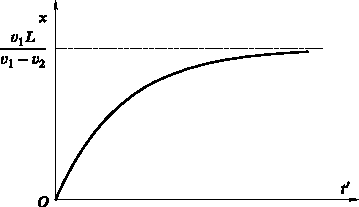
\includegraphics{figure/figa01.01}
  \caption{}
  \label{figa:01.01}
\end{figure}

\answer (1) 鸟往返了无穷多次

(2) 鸟共飞行了1秒,飞行距离为60公里

(3) $\displaystyle t= \sum_{h=0}^{t''-1} \Big(\dfrac{L}{v_{2}+v_{1}}\Big)\Big(\dfrac{v_{2}-v_{1}}{v_{2}+v_{1}}\Big)^{n}$\\
其中$ v_2 $为小鸟速率;$ v_1 $为火车速率

所以得变换为
$\displaystyle t=\dfrac{2}{3} \sum_{n=0}^{t'' -1}\Big(\dfrac{1}{3}\Big)^{n}$

\answer $ \Delta s = 5 . 0 2 $米,方向东偏北$ 284^{\circ} $

\answer (1) 位移$ 1.73 $米;路程$ 4.19 $米;平均速度$ D=0.41 $厘米/秒,方向沿
位移方向;瞬时速度为$ v=1.0$厘米/秒,方向沿圆在该点的切线

(2)位移$ 2.0 $米;路程$ 3.14 $米;$ v = 0.64 $厘米/秒,方向沿位移方向
瞬时速度$ v = 1.0 $厘米/秒,方向沿圆在该点的切线方向

\answer (1) $ 61.0 $厘米/秒,$ 60.1 $厘米/秒,$ 60.01 $厘米/秒

(2) $ 60.0 $厘米/秒

(3) $ v = 2 0 t $ , $ a = 2 0 $

\answer (1) $ - 0 .5 $米,$ -0.5 $米/秒

(2) $ 3 $米/秒,$ -6 $米/秒

(3) $ 2.25 $米

(4) $ -9 $米/秒\textsuperscript{2},$ 3 $米/秒\textsuperscript{2},$ -3 $米/秒\textsuperscript{2}

\answer (1) $\sqrt{52}$米/秒

(2) $ 20 $米/秒

\stepcounter{answer}
\answer (1) $ 1 \text{秒差距} = 3 . 0 8 5 7 \times 1 0 ^ { 1 6 } \text{米} = 2 0 6. 2 6 5 \text{AU} = 3 . 2 6 1 6 \text{光年}$

(2) $1 \text{AU} = \dfrac { 1 } { 2 0 6 2 6 5 } \text{秒差距} = 4 . 8 5 \times 1 0 ^ { - 8 } \text{秒差距}$

\answer $ t = 7 . 0 $秒, $ h = 2 4 0 $米

\answer (1) $ 27.4 $公里

(2) $ 166 $秒

\answer (1) $ 2.25 $秒

(2) 两物在地面上相遇,或不会相遇

\answer (1) $ t = 1 . 5 $秒时,$ \alpha = 1 4 ^ { \circ } 4 1 '$; $ t = 2 . 5 $秒时,$ \alpha = - 3 5 ^{\circ} 4 1' $

(2) 经过$ 0.75 $秒,高度$ h = 1 0 $米

(3) $ R _ { 1 } = 1 0 . 2 $ 米

(4) $ R _ { 2 } = 8 2 $米

\stepcounter{answer}
\answer $ v _ { 0 1 } = 2 2 . 8 $米/秒; $ v _ { 0 2 } = 2 3 . 9 5 $米/秒

\answer (1) $ \alpha = 2 5 ^ { \circ } $ 或$6 5 ^ { \circ } $

(2) $ \alpha = 4 5 ^ { \circ } $

\answer (1) 取$ O $为原点,$ x $轴竖直向下,则
$ x = - \dfrac { 1 } { 2 } g t ^ { 2 } $

(2) $ R = v _ { 0 } t $

\stepcounter{answer}
\answer $ 96 $厘米

\stepcounter{answer}
\answer $ 1.82 $公里

\answer (1) $ 1 6 9 $米/秒

(2) $ 509 $米
(3) 速率$ v = 2 1 0 $ 米/秒,与水平方向夹角$ \alpha = 61^{\circ} $

\answer $ v = \dfrac { n } { 2 } \sqrt { 2 g h } $

\answer (1) 应沿77°32的纬线自东向西飞行

(2) 可以看见太阳从西向东移动

\answer $ R _ { \text{min} } = 2 2 8 $米

\answer (1) $ \omega = 2 0 $弧度/秒
(2) $ A $点轨迹的参数方程是如下的摆线
\begin{align*}
  x      & = r \left( \omega t - \sin \omega t \right) \\
  y      & = r \left( 1 - \cos \omega t \right)        \\
  v      & = 0 . 5 \text{米}                            \\
  \omega & = 2 0 \text{弧度/秒}
\end{align*}

\answer (1) 球心速度v与球滚动的角速度a的关系为
\begin{equation*}
  v = \omega \sqrt { r ^ { 2 } - \left( d \operatorname{/} { { 2 } } \right) ^ { 2 } }
\end{equation*}

(2) 球面上任一点的轨迹均为摆线

\achapter

\stepcounter{answer}
\answer 取$ x $轴沿飞机航向,$ y $轴竖直地指向地面

(1) 取发射点为原点,炮弹轨迹方程为

$    y = \dfrac { g x ^ { 2 } } { 2 \left( v _ { 0 } + v \right) }$


(2) 取发射点为原点,炮弹轨迹方程为

$    y = \dfrac { g x ^ { 2 } } { 2 v ^ { 2 } }$

(3) 取炮弹质心为原点,飞机发射点之轨迹方程为

$    y = - \dfrac { g x ^ { 2 } } { 2 v ^ { 2 } }$

\answer $ | \vec{v} | = 2 1 . 6   $公里,与水平的车行方向夹角为 $ \theta = 7 3 ^ { \circ } 5 4 ^ { \prime }   $,如图所示
\begin{figure}[h]
    \vspace{-1.5em}
    \centering
    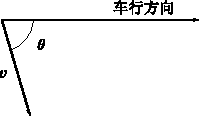
\includegraphics{figure/figa02.01}
    \caption{}
    \label{figa:02.01}
    \vspace{-0.8em}
\end{figure}

\stepcounter{answer}
\answer 水流速率$  v = 5 . 0   $公里/时

\answer (1) $ \varphi _ { 1 } = tg ^ { - 1 } \dfrac { v _ { 0 } } { v _ { 1 } }   $

(2) $ \varphi _ { 2 } = \tg ^ { - 1 } \dfrac { v _ { 0 } } { t _ { 1 } + v _ { 2 } }  $

(3) $ v ^ { \prime } = \sqrt { v _ { 1 } ^ { 2 } + v _ { 2 } ^ { 2 } }, v'' = \sqrt { \left( v _ { 1 } + v _ { 2 } \right) ^ { 2 } + v _ 0 ^ { 2 } }  $

\answer (1) $ | \vec{v} | = \sqrt { u ^ { 2 } + {v'} ^ { 2 } } = 2 0 4   $公里/时
\begin{equation*}
    \alpha = \tg ^ { - 1 } \frac { u } { v' } = 1 1^\circ 30'
\end{equation*}

(2) $ | \vec{v} | = \sqrt { {v'} ^ { 2 } - u ^ { 2 } } = 1 9 5 . 9 6 \approx 196 $公里/时
\begin{equation*}
    \theta = \sin ^ { - 1 } \dfrac { u } { v } = 1 1 ^ { \circ } 3 0 '
\end{equation*}\vspace{-1.5em}
\begin{figure}[h]
    \centering
    \subfigure[]{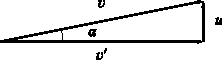
\includegraphics{figure/figa02.02a}}
    \qquad
    \subfigure[]{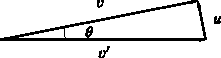
\includegraphics{figure/figa02.02b}}
    \vspace{-1em}
    \caption{}
    \label{figa:02.02}
\end{figure}\vspace{-1em}

\answer $ t _ { 0 } = \dfrac { 2 L } { u } $

% 381.jpg

(1) $ t _ { 1 } = \dfrac { t _ { 0 } } { 1 - v ^ { 2 } \operatorname{/} u ^ { 3 } }   $

(2) $ t _ { 2 } = \dfrac { t _ { 0 } } { \sqrt { 1 - v ^ { 2 } \operatorname{/} u ^ { 2 } } }  $

(3) $t_{3}=\dfrac{t_{0}}{\sqrt{1-\dfrac{v^{2}}{u^{2}} \sin ^{2} \theta \Big[1-\dfrac{v^{2}}{u^{2}}\cdot \dfrac{\cos^2\theta}{ 1-\left(v^{2} \operatorname{/} u^{2}\right) \sin ^{2} \theta}\Big]}}$

\answer $ t = 0 . 3 7 $ 秒,与参考系的选取无关

\answer $ \theta = \tg ^ { - 1 } \dfrac { 2 g h } { v }   $

\answer  $ 5 \times 1 0 ^ 8$年

\answer (1) $ v _ { A B } = v _ { A } + v _ { B }  $

(2) $ v _ { A B } = 1 . 4 c $

(3) 不违反。狭义相对论只是说,在任一惯性系中,光速不变。换一
句话说,即:若以此两物之一为参考系,要知另一物的速度就要用相
对论的速度合成公式

(4) $ v ^ \prime _ { B } \ne v _ { A B } $

\answer (1) $ 0.87 l $

(2) $ 1 . 1 5 \Delta t $

\answer $ v = 0 . 9 9 9 8 c   $

\answer $  \Delta \tau _ \text{赤极} = 1 . 8 8 4 3 \times 1 0 ^ { 5 } \text{秒} = 2 . 1 8 0 9  \text{天}= 5 . 9 7 5 0 \times 1 0 ^ { - 3 } \text{年} $

\answer $  \Delta \tau _ \text{月地} = 9.12 \times 1 0 ^ { 5 } \text{秒} = 10.55  \text{天}= 2.89 \times 1 0 ^ { - 2 } \text{年} $

\answer $  \Delta \tau _ \text{日地} = 7.75 \times 1 0 ^ { 5 } \text{秒} = 8.979 \text{天}= 2.46 \times 1 0 ^ { - 2 } \text{年} $

\answer $ \tau = \dfrac { \tau _ 0 } { \sqrt{ 1 - v ^ { 2 } \operatorname{/} c ^ { 2 } } } $

\answer $ \tau = 1 0 \tau _ { 0 } = 2 2   $微秒

\achapter

\answer $ F _ { \text{min} } = 1 4 4 $公斤力

\answer $ 15 $吨

\answer $ 25 $公斤力
% 382.jpg

\answer $ 10 $米/秒

\answer $ 5.91 $米

\answer (1) $ 50 $公斤

(2) 上升时,$ 75 $公斤;下降时,$ 25 $公斤

\answer (1) $ \left( M - m \right) g $

(2) $ \left( M - m \right) g - m a $

\answer (1) $ 98 $厘米/秒

(2) $ 17.6 $牛顿

\answer $ \mu = \dfrac { m _ { B } \left( g - a \right) - m _ { A } a } { m _ { A } g } $

\answer $ \dfrac { F _2 }{ F _1 } = \dfrac { 1 } { \cos \alpha - \mu \sin \alpha } $


\answer (1) $ 4.0\text{吨力} \approx 39.2 \times 10 ^ 3 \text{牛顿} $

(2) $ 4.0\text{吨力} \approx 39.2 \times 10 ^ 3 \text{牛顿} $

(3) $ 4.0\text{吨力} \approx 39.2 \times 10 ^ 3 \text{牛顿} $

(4) $ 40.8 \times 10 ^ 3 \text{牛顿} \approx 4.1 \times 10 ^ 4 \text{牛顿} $

(5) $ 3.6 \times 10 ^ 4 \text{牛顿} $

(6) $ 2.45 $米/秒

\answer $ m_2 $在桌上时,加速度$ a = 4 . 9 $米/秒\textsuperscript{2},张力$ T = 1 . 4 7 $牛顿;

$ m_1 $在桌上时,加速度$ a = 2 . 4 5 $米/秒,张力$ T=1.47 $牛顿

\answer $ a = \dfrac { m g - \mu \left( m _ { 1 } + m _ { 2 } + m _ { 3 } \right) g } { m + \left( m _ { 1 } + m _ { 2 } + m _ { 3 } \right) } $

$ T _ { 1 } = m _ { 1 } \left( a + \mu g \right) $

$ T _ { 2 } = \left( m _ { 1 } + m _ { 2 } \right) \left( a + u g \right) $

$ T _ { 3 } = m \left( g - a \right) $

\answer $ a = \dfrac { m _ { 1 } \sin \alpha -m _ { 2 } } { m _ { 1 } + m _ { 2 } + m _ { 3 } } g $

$ T _ { 1 } = m _ { 1 } \left( g \sin \alpha - a \right) $

$ T _ { 2 } = m _ { 2 } a $

取$ x $轴向右,$ y $轴向上,则得$ A $点承受之支持力为

$ \vec{N} = \vec{i} N _ { x } + \vec{j} N _ { y } $

% 383.jpg
$ N _ { x } = T _ { 1 } \cos \alpha $

$ N _ { y } = T _ { 1 } \sin \alpha + T _ { 2 } $

$ B $点拉滑轮的绳$ d $承受的张力$ T = \sqrt { 2 } T _ { 2 } $

\answer $ \mu _ { 0 } = 0 . 5 7 7$ , $\mu = 0 . 5 3 0 $

\answer (1) $ F = \left( M + m \right) g \tg \alpha $

(2) $ a = g \tg \alpha $

\answer (1) $ m g - \beta v = m a $

\aindent $ m g - \beta \dot{z} = m \ddot{z} $

(2) $ v \left( t _ { 0 } \right) = \dfrac { m } { \beta } g $

(4)略

\answer (1) $ g \sin \theta $,沿斜面向下

(2) $ g \sin \theta $,沿斜面向下

(3) $ \left( g - a \right) \sin \theta $,当$ g > a $时沿斜面向下

\aindent 当$ g < a $时沿斜面往上

\aindent 当$ g = a $时物与斜面相对静止

(4) $ \left( g + a \right) \sin \theta $,沿斜面向下

(5) 0

(6) $ m \left( g - a \right) \cos \theta $

\stepcounter{answer}
\answer $ a _ { 1 } = \dfrac { 3 } { 7 } g $向下

$ a _ { 2 } = \dfrac { 1 } { 7 } g$,向上

$ a _ { 3 } = \dfrac { 1 } { 7 } g $,向上

$ T _ { 1 } = 2 . 2 3 $牛顿

$ T _ { 2 } = - 4 . 4 6 $牛顿

\answer $ a _ { 2 } = 97.4 $米/秒

\answer $ \mu _ { \text{min} } = 0 . 3 9 4 $

\answer 张力$ T = \dfrac { M g } { 2 \uppi } \ctg \dfrac { \alpha } { 2 } $

% 384.jpg
\answer (1) $ v _ { 0 } = \sqrt { l g } = 1 9 8 $ 厘米/秒

(2) $ T = 3 m g = 2 . 9 4$牛顿

\answer (1) $v=\sin \theta \sqrt{\dfrac{l g}{\cos \theta}}=\sqrt{g l \tg \theta \sin \theta}$

\makebox[1.5em]{}$ F = m g \tg \theta $

\answer $ h = R - \dfrac{ g }{\omega ^ 2} $ ,或在碗底不动

\answer (1) $ v = \sqrt { g h } $

(2) $\sqrt{g h \dfrac{1-\mu \operatorname{tg} \theta / 2}{1+\mu c \operatorname{tg} \theta / 2}} \leqslant v \leqslant \sqrt{g h \dfrac{1+\mu \operatorname{tg} \theta / 2}{1-\mu \operatorname{ctg} \theta / 2}}$

\answer $\sqrt{R g \dfrac{\sin \alpha-\mu \cos \alpha}{\cos \alpha+\mu \sin \alpha}} \leqslant v \leqslant \sqrt{R g \dfrac{\sin \alpha+\mu \cos \alpha}{\cos \alpha-\mu \sin \alpha}}$

若$ v < \sqrt{R g \dfrac{\sin \alpha-\mu \cos \alpha}{\cos \alpha+\mu \sin \alpha}} $,则车往里倒或下滑

若$ v > \sqrt{R g \dfrac{\sin \alpha+\mu \cos \alpha}{\cos \alpha-\mu \sin \alpha}} $,则车往外倒或往外跑

若$ \mu = 1 $且$ \theta = \uppi / 4 $,则任何速率都可安全行驶

\answer (1) $ \dfrac { W } { 2 \cos \theta } $

(2) $ \dfrac { W } { 2 } \tg \theta $

\answer (1) $ T \left( \theta \right) = \lambda R g \sin \theta $

(2) $ N \left( \theta \right) \Delta \theta = 2 \lambda R g \sin \alpha \cdot \Delta \theta $
\begin{figure}[h]
  \centering
  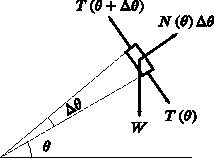
\includegraphics{figure/figa03.01}
  \caption{}
  \label{figa:03.01}
\end{figure}

$\sum N _ {\text{水平}} = \displaystyle \int_{0}^{\frac{\pi}{2}} N(\theta) \cos \theta d \theta=\lambda P g=T\left(\dfrac{\pi}{2}\right)=T_{A}$\\
这是绳的平衡条件

\answer (1) $ a = \dfrac y L { g } $\vspace{-0.5em}

(2) $ y \left( t \right) = y _ { 0 } \ch \sqrt { \dfrac g L } t $

\answer $ T = M \omega ^ { 2 } l \big/ \left( 2 \uppi \right) ^ { 2 } $

\answer (1)
\begin{figure}[h]
  \vspace{-0.8em}
  \centering
  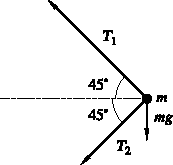
\includegraphics{figure/figa03.02}
  \caption{}
  \label{figa:03.02}
  \vspace{-0.8em}
\end{figure}

(2) $ T _ { 1 } = \dfrac { 1 } { 2 } \left( m \omega ^ { 2 } l + \sqrt { 2 } m g \right) $

\aindent $ T _ { 2 } = \dfrac { 1 } { 2 } \left( m \omega ^ { 2 } l - \sqrt { 2 } m g \right) $

\answer $ T _ { A } \big/ T _ { B } = e ^ { - \mu \theta } $

\answer (1) 图略

(2) $\begin{cases}T-m_{1} g=m_{1} a \\ m_{2} g \sin \theta-T=m_{2} a \\ N-m_{2} g \cos \theta=0\end{cases}$

\aindent $T=\dfrac{m_{1} m_{2} g(1+\sin \theta)}{m_{1}+m_{2}}$

\aindent $a=\dfrac{\left(m_{2} \sin \theta-m_{1}\right) g}{m_{1}+m_{2}}$

(3) $\mu_{\text { min }}=\dfrac{\cos \theta\left(m_{2} \sin \theta-m_{1}\right)}{m_{1}(1+\sin \theta)^{2}+\left(m_{1}+m_{2}\right)\left(M \operatorname{/} m_{2}+\cos ^{2} \theta\right)}$

% 386.jpg
\answer $\Bigl(\dfrac{\sin \theta-\mu \cos \theta}{\mu \sin \theta+\cos \theta}\Bigr) g \leqslant a \leqslant\Bigl(\dfrac{\sin \theta+\mu \cos \theta}{\cos \theta-\mu \sin \theta}\Bigr) g$

\answer 拱形、桥受压力 $ N = m g \cos \theta - m v ^ { 2 } \operatorname{/} R $

凹形,桥受压力$ N = m g \cos \theta + m v ^ { 2 } \operatorname{/} R $

\achapter

\answer (1) $G=\dfrac{\kappa \theta r^{2}}{M m l}$

(2) $ 6 . 6 3 \times 1 0 ^ { - 1 1 } $牛顿$ \cdot $米/公斤\textsuperscript{2}

\answer $ F_\text{日月} \approx 6 \times 1 0 ^ { 32 }$牛顿

$ F_\text{地月} \approx 3 \times 1 0 ^ { 32 }$牛顿

\answer $ 3 . 4 6 \times 1 0 ^ { 5 } $公里

\answer {\ziju{-0.05pt}引力大小为$ \dfrac { 2 G \rho M } { x } $,
  方向沿由$ M $向直线所作竖直垂线的方向}

\answer (1) $ \dfrac{G m_{1} M}{x \sqrt{L^{2}+x^{2}}}$
,方向从$ m_1 $指向原点

(2) $G m_{2} \rho\Bigl(\dfrac{1}{y-L}-\dfrac{1}{y+L}\Bigr)=G m_{2} \dfrac{M}{2 L}\Bigl(\dfrac{1}{y-L}-\dfrac{1}{y+L}\Bigr)$,
方向沿直线

(3) 约$ 1 . 7 \times 1 0 ^ { - 1 0 } $达因

\stepcounter{answer}
\answer (1) $\dfrac{G M_{1} M r}{R_{0}^{3}}$

(2) $\Bigl(\dfrac{G M_{1} M r}{R_{0}^{3}}\Bigr) ^ {\frac {1}{2}}$


\answer 重9.96公斤

\answer (1) $ \rho _ { m } \operatorname{/} \rho _ { e } = 0 . 7 3 $

(2) $ g_\text{火星}=3.7 $米/秒

\answer $ M _ { e } \approx 5 . 9 8 \times 1 0 ^ { 24 } $公斤


\answer $ M _ \text{日} = \dfrac { 4 \uppi ^ { 2 } r ^ 3 } { G T ^ { 2 } } = 1.97 \times 1 0 ^ { 33 } \text{克} = 1.97 \times 10 ^ { 30 }$公斤

% 387.jpg
\answer $ n \approx 6 . 5 \times 1 0 ^ { 1 0 } $个

\answer $F=\dfrac{G M m}{d^{2}}\Bigl[1-\dfrac{1}{8(1-R \operatorname{/} 2 d)^{2}}\Bigr]$,
方向从$ m $指向铅球球心

\stepcounter{answer}
\answer $ h = 2 8 0 $公里

\answer (1) 同步卫星轨道平面必须在赤道平面内

(2) $ r \approx 4 . 2 \times 1 0 ^ { 4 } $公里$ \sim 7 R_0 $,$ R_0 $为地球半径

\answer (1) $ \rho \geqslant \dfrac { \omega ^ 2 } { \dfrac { 4 \uppi } { 3 } G } $

(2) $ \rho _ \text{最小} = 1 . 3 \times 1 0 ^ { 11 }$克/厘米$ =1.3\times 10 ^ { 14 } $公斤/米

(3) $ R_\text{最小} \approx 150 $公里

(4) $ R \approx 17 $公里

\answer $ 3 R _ { 0 } $, $ R _ { 0 } $ 为地球半径

\answer $ M > 1 . 3 5 R \times 1 0 ^ { 23 } $克,其中$ R $以厘米为单位

\answer $ R < 1 . 4 7 $公里

\answer (2) $ 30.2 $公里/秒

\answer (1) $ 4.83 $天
(2)$ 64.6 $天

\answer $ 5 . 3 6 \times 1 0 ^ 9 $公里

\achapter

\answer $1+\Bigl[\dfrac{R(t)}{R_{0}}\Bigr]^{3}-2\Bigl[\dfrac{R(t)}{R_{0}}\Bigr]^{\frac{3}{2}}=6 \pi G \rho_{0}\left(t-t_{0}\right)^{2}$ \\
式中$  t _ { 0 }   $表示现在的时刻,$ \rho _ 0 $及$ R _ 0 $分别是$  t _ { 0 }   $时刻的平均密度及宇宙尺
度因子\vspace{-0.25em}

\answer 因为
$\dfrac{\dif^{2} R(t)}{\dif t^{2}}=-\dfrac{4 \pi G}{3}\cdot\dfrac{\rho_{0} R_{0}^{3}}{R_0}<0,\dfrac{\dif}{\dif t}\Bigl[\dfrac{\dif R(t)}{\dif t}\Bigr]<0$\\
所以是减速的

\achapter

\answer $ 58 $公斤力,$ 5.0\times 10^2 $公斤米,或$ 4.9\times 10 ^3$焦耳

% 388.jpg
\answer $ (1) 11.76\times 1 0 ^ { 5 } $焦耳

(2) $ 0.44 $马力

\answer $ 1 . 2 3 \times 1 0 ^ { -2 } $马力

\answer $ P = 2 3 . 2 5 $瓦,能量为$ 2.01\times 10 ^ 6 $焦耳

\answer $ 17 $秒

\answer $ 6 \times 1 0 ^ { - 2 } $米

\answer $ m g L \operatorname{/} 2 $

\answer $ 4 . 2 \times 1 0 ^ { 6 } $焦耳

\answer $ 156 $千瓦

\answer $ -22.5 $公斤$ \cdot $米

\addtocounter{answer}{2}
\answer 下落速度$v=\sqrt{g\Bigl(L-\dfrac{a^{2}}{L}\Bigr)}$

\answer $ v = 1 2 . 1 $厘米/秒


\answer $ v _ { 0 } = 7 . 1 $米/秒

\answer
$ v _ { \text{max} } = \dfrac { m _ { 2 } g } { \sqrt { m _ { 1 } k } } $

\answer $ \overline { F } = 1 2 2 0 0 $牛顿$ \approx 1.2\times 10 ^ 4 $牛顿

\answer (1) $ E _ { k 0 } = 1 8 . 6 $焦耳, $ E _ { pt } = 9 . 8 $焦耳

(2) $ f _ { \mu } = m g \sin 3 0 ^ { \circ } = 0 . 4 9 $牛顿

(3) 不会再往回滑,所以$ t = \infty $

\answer (1) $ - m g r \left( 1 - \cos \theta \right) $

(2) $ m g r \left( 1 - \cos \theta \right) $

(3) 径向为$ 2 g \left( 1 - \cos \theta \right) $,切向为$ g \sin \theta $

(4) $ \theta = \cos ^ { - 1 } \left( 2 / 3 \right) $

\answer (1) $ v _ { \text{min} } = \sqrt { 5 g R } $

(2) $ \theta = 1 9 ^ { \circ } 3 0 ^ { \prime } $或 $ \theta = \sin ^ { - 1 } \left( 1 \operatorname{/} 3 \right) $

\answer (1) $ v _ { B } = \sqrt { 2 g \left( h - R \right) } $,$ F _ { B } = \dfrac { 2 m g \left( h - R \right) } {R} $,
$ N _ { B } = \dfrac { 2 m g h } { R } - 3 m g $

% 389.jpg
(2) $ h \geqslant 1 . 5 R $

\clearpage
\answer $ \theta = \cos ^ { - 1 } \Bigl( \dfrac { 1 } { 8 } + \sqrt { \dfrac { 1 } { 9 } - \dfrac { M } { 6 m } } \Bigr) $

\answer (1) 绳渐伸长。在弹性限度内,升降机的动能转化为绳的弹性势能
及升降机的势能变化

(2)绳上最大张力$ T_\text{max}=9.3 $吨力伸长量$ \Delta x = 8 . 3 $厘米

\answer $ \dfrac { M } { M - m } l $

\answer $ 11 $倍

\answer 取无穷远处为势能的零点

$ r > R,~ U \left( r \right) = - \dfrac { G M } { r }$

$ r < R,~ U \left( r \right) = - \dfrac { 3 } { 2 } \cdot \dfrac { G M } { R } + \dfrac { 1 } { 2 } \cdot \dfrac { G M } { R ^ { 2 } } r ^ { 2 } $

\stepcounter{answer}
\answer (1) $ v _ \text{逃} = \sqrt { 2 } v _ { 0 } $

(2) 达$ R_0 $,则$ v _ { 1 } = v _ { 0 } $;达$ \dfrac { 1 } { 2 } R _ { 0 } $,则$ v _ { 3 } = - \dfrac { 1 } { 3 } v _ { 0 } $

(3) $v\left(R_{0}+y\right)=-m v_{0} 2\Bigl[1-\dfrac{y}{R_{0}}+\Bigl(\dfrac{y}{R_{0}}\Bigr)^{2}+\cdots\Bigr]$

(4) $v_{\text{min}}=\sqrt{2\Bigl(\dfrac{v_{0}^{2}}{R_{0}}\Bigr) y\Bigl(1-\dfrac{y}{R_{0}}\Bigr)}$,

或$v_{\text{min}} = \sqrt { 2 y g _ { 0 } } $

\stepcounter{answer}
\answer $ 9 . 6 \times 1 0 ^ { 7 } $秒

\answer (1) $ \sqrt { 2 g R _ { e } } $,$ R_e $为地球半径

(2) $ m r + k \dot{r} - \dfrac { G M m } { r ^ { 2 } } = 0 $,取地心为坐标原点,$ r $为流星与地心之距离

(3) $ \dfrac{g m}{k} $

\answer (1) $ 5 . 7 5 \times 1 0 ^ { 16 } $焦耳

(2) $ 5.87\times 10 ^9 $吨

% 390.jpg
\answer $ 2 . 2 3 \times 1 0 ^ { 3 } $吨/秒

\achapter

\answer $ T = 0 . 7 3   $秒

\answer 在竖直方向

\answer 相同

\answer $ \varphi _ { 0 } = 0   $

\answer (1) $ \dot{y} = A \omega \cos \omega t + 2 \omega \cos 2 \omega t$

\aindent $ \dot{y} = - A \omega ^ { 2 } \sin \omega t - 4 \omega ^ { 2 } \sin 2\omega t   $

(2)不是

\addtocounter{answer}{2}
\answer (1) $ \nu = 1 .  5 $赫兹

(2) $ A = 2 . 2 $厘米

(3) $  \varphi _ { 0 } = 2 4 ^ \circ 3 7 ^ { \prime } = 0 . 4 3 $ 弧度

(4) $ x = \sqrt { 5 } \cos \left( 7 \sqrt { 2 } t + 0 . 4 3 \right)  $

\answer $  T = 2 . 2 1   $秒

\answer $t=\pm \dfrac{\pi}{4 \omega}-\dfrac{\varphi_{0}}{\omega}+\dfrac{n \pi}{\omega}, n=0, \pm 1, \pm 2, \ldots$

\answer $ T = 0 . 7 7 $秒

\answer $ m = 1 .  6 $公斤

\answer (1) 振幅$  A \geqslant 2 4 . 8 3   $厘米时

(2) $ \nu _ {\text{max}} = 2 . 2 3   $赫兹

\answer $ A _ { \text{max} } = 3 . 1   $厘米

\answer $ 120^{\circ} $

\answer (1) $ 14 $牛顿/米

(2) $ M = 7 9   $克

\answer $ k _ { 1 } = \dfrac { n + 1 } { n } k , k _ { n } = \left( n + 1 \right) k  $

\answer $ \nu = \dfrac { 1 } { 2 \uppi } \sqrt { \dfrac { k _ { 1 } + k _ { 2 } } { m } }  $

\answer $ C $点为质心,不动,图\ref{fig:07.17} 中有$  m _ { 2 } l _ { 2 } = m _ { 1 } l _ { 1 }  $

    % 391.jpg
$ m _ 2 $对质心作简谐振动,振动方程为

$x_{2}=l_{2}+(l_{2}^{\prime}-l_{2}) \cos \omega_{2} t,\quad \omega_{2}=\sqrt{\dfrac{k(m_{1}+m_{2})}{m_{1} m_{2}}}$

$ m_1 $对质心作简谐振动,振动方程为

$x_{1}=-l_{1}+(l_{1}^{\prime}-l_{1}) \cos \omega_{1} t, \quad \omega_{2}=\omega_{2}$

\answer $ C $点作自由落体运动,$  m _ { 1 }, m _ 2 $相对$ C $的运动同上题

\answer (1) $ T = 2 \uppi \sqrt { \dfrac { l _ { 1 } ^ 2 + l _ { 2 } ^ 2 } { ( l _ { 1 } - l _ { 2 } ) g } } = 1 . 7$秒

(2) $ l _ { 0 } = 7 5   $厘米

\stepcounter{answer}
\answer $ 75 $公里/时

\answer $ Q \approx 7,0 0  0 $

\answer $ Q \approx 1 3   $
\achapter

\answer $ x _ { c } = 1 3   $厘米, $ y _ { c } = 8   $厘米

\answer  $ x _ { c } = - 0 . 1   $米, $ y _ { c } = 0 .1   $米

\answer {\ziju{-0.05pt}取$ x $轴在二圆心联线且从圆盘中心指向孔中心的方向,取盘中心为原
点,$ y $轴过原点与$ x $轴垂直,则得$  x _ { c } = - 5 . 6   $厘米,$ y _ { c } = 0  $}

\answer $  x _ { c } = 0 ,~ y _ { c } = - \frac { 2 a } { 8 \uppi } $

\answer (1) 气球向下运动,速率为$ \dfrac { m v } { M + m }  $

(2) 气球静止

\answer $ 2.6 $米

\answer $ 4900 $公里

\answer 取两球心联线为$ x $轴,$  m _ 1 $ 球心为原点,则:

(1) $ x _ { c } \left( 0 \right) = 0 . 2 5   $米

(2) $  a _ { c } = 2 g  $

(3) $ x _ { c } \left( 3 \right) = 8 8   $米

(4) $ E _ { 0 } = 8 . 9 \times 1  0 ^ 4 $焦耳

(5) $ E ^ { \prime } = 3 . 1 \times 1 0 ^ 4 $焦耳

% 392.jpg
\stepcounter{answer}
\answer (1) $ \vec{a} _ { 1 } = 3 . 5\vec{i}    $米/秒\textsuperscript{2}, $ \vec{a} _ { 2 } = 2\vec{j}  $米/秒\textsuperscript{2},$ \vec{a} _ { 3 } = -1.5\vec{i} $米/秒\textsuperscript{2}

(2) $ \vec{r} _ { c } \left( 0 \right) = \left( 1 . 7 5 , 0 . 2 5 \right)  $

(3) $ \vec{a} = 0 . 5\vec{i} \text{米/秒\textsuperscript{2}}+1\vec{j}\text{米/秒\textsuperscript{2}}$

\answer (1) $ v _ { A } = 5 8 .  6 $米/秒, $ v _ { B } = 4 1. 4   $米/秒

(2) $ 20\% $

\answer $ f = 4 0  $ 牛顿

\answer (1) $ F / A = 1 . 8 \times 1 0 ^ 4  $牛顿/厘米\textsuperscript{2},会骨折

(2 $ F / A = 3 . 6 \times 1 0 ^ 2  $牛顿/厘米\textsuperscript{2},不会骨折

\answer $ 600 $米/秒

\answer 大于$ 0.86 $公斤$ \cdot $米/秒

\answer $ 2 . 4 \times 1 0 ^ { 5 }   $米/秒\vspace{-0.5em}

\answer  (1) $ \left( m _ { 1 } + m _ { 2 } \right) g + \dfrac { 2 m _ { 1 } ^ 2 } { m _ { 1 } + m _ { 2 } } g  $\vspace{-0.5em}

(2) $ \Bigl( \dfrac { m _ { 1 } } { m _ { 1 } + m _ { 2 } } \Bigr) ^ { 2 } R   $

\stepcounter{answer}
\answer (1) 取$ \vec{v} _ 1 $为正方向,则碰后$  \vec{v} _ { 1 } ^ { \prime } = 0   $, $ \vec{v} _ { 2 } ^ { \prime } = 1 6   $厘米/秒

(2) 取$ \vec{v} _ 1 $为正方向,碰后共同的速度$  v = 6   $厘米/秒

\answer (1) 车向右加快,$  \Delta v = 2 . 7   $米/秒

(2) 车速与他未跳下时同,仍为$ 12.7 $米/秒

\answer (1) 向右,速率为$ 4.5 $米/秒

(2)向右,速率为$ 3.5 $米/秒

\answer (1) $ v = v _ { 0 } + \sum _ { a = 1 } ^ n \dfrac { m u } { W + a m } $

(2) $ v = v _ { 0 } + \dfrac { n m u } { W + n m }  $

\answer (1) $ 8.25 \times 10 ^ 8 $米/秒

(2) $4.02\times 10 ^ 8 $米/秒

\answer 需要的力为$ \vec{F} = \left( \vec{v} - \vec{u} \right) \dfrac { \dif m } { \dif t } $

\answer 最终速率$  v = \sqrt { g \operatorname{/} k }  $
% 393.jpg

\answer $\frac{x^{2}}{\left(\frac{M}{M+m}\right)^{2} R^{2}}+\frac{y^{2}}{R^{2}}=1 $

\answer (1) $ F = \frac { \dif m } { \dif t } v   $,功率$  P = \frac { \dif m } { \dif t } v ^ { 2 }  $

(2) $ \dfrac { 1 } { 2 } $转变成砂子的动能,其余由于滑动摩擦,变成热能消耗

(3) 没有改变

\addtocounter{answer}{2}
\answer $ N = \left( M + m \right) g + m g \sqrt { 1 + \dfrac { 2 k h } { g \left( M + m \right) } }   $

\answer (1) $v_{A}=\sqrt{\dfrac{2 M^{2} g h \cos ^{2} \theta}{(M+m)\left(M+m \sin ^{2} \theta\right)}}$

\aindent $\vec{v}_{A}=\sqrt{\dfrac{2 m^{2} g h \cos ^{2} \theta}{(M+m)\left(M+m \sin ^{2} \theta\right)}}$

\aindent $v_{B}=\sqrt{\dfrac{2 M g h}{M+m}}$

\aindent $\vec{v}_{B}=\sqrt{\dfrac{2 m^{2} g h}{M(M+m)}}$

(2) $\Delta E_{A}=m g h\Bigl(1-\dfrac{M \cos ^{2} \theta}{M+m \sin ^{2} \theta} \Bigr)$
,这部分能量是$ m $与桌面在竖
直方向发生完全非弹性碰撞损失的

\aindent $ \Delta E _ { B } = 0   $

\answer (1) $ v _ { c0 } = \sqrt { 2 g H }   $,方向沿$ AC $方向

(2) $ v _ { c } = U _ { c0 } \cos \theta  $ ,方向沿水平即$ CD $方向

(3) $ \Delta P = m v _ { y } = m \sqrt { 2 g H } \sin \theta = m v _ { c0 } \sin \theta $,方向竖直向下

$ \Delta E = \dfrac { 1 } { 2 } m v _ { c0 } - \dfrac { 1 } { 2 } - m v _ { c } ^ { 2 } = m g H \sin ^ { 2 } \theta  $,  这是由于在竖直方向和地
面的完全非弹性碰撞而损失的能量

\answer (1) $ s = \dfrac { h } { \mu } \left( 1 - \mu \ctg \theta \right) \left( 1 - \sin ^ 2 \theta - 2 \mu \sin \theta \cos \theta + \mu ^ { 2 } \sin ^ { 2 } \theta \right) $

(2) 当$ \theta  $很小时%\vspace{-1em}
% 394.jpg
\begin{align}
    &s \approx \frac { h } { \mu } \left( 1 - \mu \ctg \theta \right)  \tag{i} \\[-0.5em]
    &\ctg \theta = \frac { s _ { 0 } } { h }  \tag{ii}
\end{align}

第六章习题11结果是$ s + s _ { 0 } = \dfrac { h } { \mu }  $。
本习题上面的结果(i),(ii)联合,即得
$ s + s _ { 0 } \approx \dfrac { h } { \mu } - h \ctg \theta + h \ctg \theta = \dfrac { h } { \mu }   $
与第六章相同

\answer  (1) $ v = \sqrt { \dfrac{ 2 } { 3 } g x }   $

(2) $ 2 \operatorname{/} 3  $

\answer (1) $ v = u \bigl( 1 - \e ^ { - \frac { m } { M } t } \bigr)  $

(2) $ \eta = 2 \left( \dfrac { u } { v } \right) \left( 1 - \dfrac { v } { u } \right)  $;$  v = \dfrac { u } { 2 }   $时,$\eta$最大, $ \eta _ { \text{max}} = \dfrac { 1 } { 2 }   $。式中$ \eta, v $都是数值

\achapter

\answer (1) $ L _ { c } = 2 m l ^ 2 \omega $,方向垂直于棍所在的平面

$ \vec{L} _ { o } = \vec{L} _ { c }   $

(2) $ L _ { c } = m R ^ { 2 } \omega   $,方向垂直于圆环的面

$\vec{L} _ { o } = \vec{L} _ { c } $

\stepcounter{answer}
\answer (1) $ \omega \left( t \right) = \omega _ { 0 } \Bigl( \dfrac { r _ { 0 } } { r _ { 0 } - v t } \Bigr) ^ { 2 }   $

(2) $F = m \dfrac { \omega _ 0 ^ { 2 } r _ 0 ^ { 4 } } { r _ { 0 } - v t } $

\answer (1) $ 3 . 9 \times 1 0 ^ { 3 } $公斤$ \cdot $米\textsuperscript{2}/秒

(2) $ 13 $米/秒

(4) $ 406 $公斤力

\answer (1) 绕粘结点(质心)转动

(2) $ \omega = \frac { 3 v } { 2 l }  $
% 395.jpg

\answer $  4 . 7 3 \times 1 0 ^ 5 $ 公里

\answer (1) $r=\dfrac{\beta^{2} R_{0}}{1+\left(\beta^{2}-1\right) \cos \varphi}$,
原点为原有的圆心,火箭爆发点相应于
$ \varphi = 0  $


(2) {\ziju{-0.05pt}飞船点火时,即火箭爆发,相应$  \varphi = 0   $,所以速度方向为$ \uppi \operatorname{/} 2 $}

$ r \to \infty $为逃逸,相应于$  \cos \varphi _ \infty = - \dfrac { 1 } { \beta ^ { 2 } - 1 }, ~ \alpha = \varphi _ \infty - \dfrac { \uppi } { 2 }  $\\[-0.5em]
所以$  \sin \alpha = - \cos \varphi _ \infty = \dfrac { 1 } { \beta ^ { 2 } - 1 }  $ \\
当$  \beta = \sqrt { 3 }  $ 时,$  \alpha = 3 0 ^ \circ  $

\answer (1) $ r = \dfrac { R _ { 0 } } { 1 + \cos \varphi } $

\answer 地球自转角动量为$ 5.23\times 10 ^ 32 $公斤$ \cdot $米/秒

\answer $\omega=\dfrac{m R^{2} v}{\dfrac{1}{2} M R_{1}^{2}+m R_{2}^{2}}$

\answer 角速度变化
$ \Delta \omega = \dfrac { m R ^ { 2 } } { I } \omega  $

能量变化 $\Delta E=\dfrac{1}{2} m R^{2} \omega^{2}+\dfrac{m^{2} R^{4}}{2 I} \omega^{2}$

\answer (1) 小球反向以$ u $运动,
$ u = \dfrac { v \left( m _ { 0 } -  3 m \right) } { m _ { 0 } + 3 m }   $

板向前方以角速度$ \omega_{ 1 } $旋转
$\omega_{1}=\dfrac{6 m v}{\left(m_{0}+3 m\right)a}$\vspace{-0.5em}

(2) $ \omega = \dfrac { 3 m v } { \left( m _ { 0 } + 3 m \right) a }   $

\answer 月-地距$  > 1 . 5 \times 1 0 ^ { 6 }   $公里时,月会飞掉

\achapter

\addtocounter{answer}{4}

\answer $ I = \dfrac { 1 } { 1 2 } m \Bigl( a ^ 2 + b ^ { 2 } - \dfrac { 2 c ^ { 4 } } { a b } \Bigr) $

\answer $ I = \dfrac { m } { 1 2 a b } \left( a ^ { 3 } b + b ^ { 3 } a - 6 \uppi r ^ { 4 } \right)  $
% 396.jpg

\answer (1) $ 1 6 \times 1 0 ^ { 4 }   $克$ \cdot $厘米\textsuperscript{2}

(2) $  1 . 2 \times 1 0 ^ { 4 }   $克$ \cdot $厘米\textsuperscript{2}

\answer $ I = \dfrac { 1 } { 2 } - m \left( R _ { 1 } ^ { 2 } + R _ { 2 } ^ 2 \right) $

\answer $ I = \dfrac { 1 } { 4 } m R ^ { 2 }  $

\answer $ I = \dfrac { m } { 12 } h ^ { 2 } + \dfrac { 1 } { 4 } m R ^ { 2 }  $

\answer $ \beta = 3 . 2 8   $弧度/秒\textsubscript{2}

\answer $ a _ { c } = \dfrac { 5 } { 7 } g \sin \alpha $

\answer $ \beta = - 2 .  1 $弧度/秒\textsubscript{2}, $ n = 7 0 . 8   $转,再经$ 40 $秒停止

\answer $ v = 2 \sqrt { \dfrac { m g h } { 2m + M } }   $

\answer $T=\dfrac{m_{1} \mu+m_{1}+M \mu}{m_{1}+m_{2}+M} g, \quad T^{\prime}=\dfrac{m_{2}+m_{2} \mu+M}{m_{1}+m_{2}+M} g$

$a=\dfrac{m_{1}-m_{2} \mu}{m_{1}+m_{2}+M} g$

\answer $ a = - \dfrac { 2 } { 3 } g $ , $ T = \dfrac { 1 } { 3 } m g $

\answer $ f = 2 9   $公斤力

\answer $v=\sqrt{\dfrac{4}{3} g h}=2 \sqrt{\dfrac{g h}{3}}$

\answer $ f = 3 . 5 9 \times 1 0 ^ { 3 }   $牛顿

\answer $a=\dfrac{4(2 M-m)}{8 M+7 m} g, \quad T_{1}=\dfrac{m g}{8 M+7 m}(5M+3 m)$

$T_{2}=\dfrac{m g}{8 M+7 m}(7 M+2 m), \quad T_{3}=\dfrac{11 M m}{8 M I+7 m} g$

\answer (1) $ a = 2 . 3 3   $米/秒\textsubscript{2}

(2) $ T_ { 1 } = 3 5 $牛顿, $ T _ { 2 } = 3 7 . 3 2   $牛顿

\answer 转了 $ \dfrac { 1 } { 2 \uppi } \sqrt { \dfrac { 3 h } { a } }  $转
% 397.jpg
\clearpage
\answer $ M = - 0 . 0 8  $牛顿$ \cdot $米,其中负号表示与原转动角动量反方向

\answer (1) $ v _ { B } = 1 2 .  1 $米/秒

(2) $ y _ { H } = 3 . 3 3$米

\answer 球先到下端,$  v _ { c \text{质点} } > v _ { c \text{球} } > v _ { c \text{柱} }$

\answer (1) $a_{c 1}=\dfrac{5}{7} g \sin \alpha, \quad v_{c 1}=\sqrt{\dfrac{10}{7} g h}, \quad \omega_{1}=20 \sqrt{\dfrac{10}{7} g h}$

\aindent $a_{c 2}=\dfrac{5}{7} g \sin \alpha, \quad v_{c 2}=\sqrt{\dfrac{10}{7} g h}, \quad \omega_{2}=10 \sqrt{\dfrac{10}{7} g h}$

\aindent $a_{c 3}=\dfrac{3}{5} g \sin \alpha, \quad v_{c 3}=\sqrt{\dfrac{6}{5} g h}, \quad \omega_{3}=20 \sqrt{\dfrac{6}{5} g h}$

\aindent $a_{c 4}=\dfrac{3}{5} g \sin \alpha, \quad v_{c 4}=\sqrt{\dfrac{6}{5} g h}, \quad \omega_{4}=10 \sqrt{\dfrac{6}{5} g h}$

(2) 同样结构的球(实或空)$ a _ c $与$ m,r $无关,
但$ \omega \propto \dfrac { 1 } { r }  $\vspace{-0.5em}

\aindent 同样的材料、同样尺寸,则$
a _ { c }, \omega \propto \dfrac { 1 } { I }  $

\answer $ t = 2 . 1 $秒

\answer {\ziju{-0.02pt}$ \omega _ { 0 } > \dfrac { 5 } { 2 } \cdot \dfrac { v _ { 0 } } { R }   $时,\!成为“来去”;$ \omega _ { 0 } = \dfrac { 2 } { 5 } \cdot \dfrac { v _ { 0 } } { R }   $,\!则同时停转又停止}

\answer $ \mu \geqslant \dfrac { 1 } { 3 } \tg \alpha   $\vspace{-1em}
\achapter

\answer $ \tau = 1 . 5 7 \times 1 0 ^ { -5 }   $秒

\answer $ v _ B ^ { \prime } = - 0 . 9 5 c  $

\addtocounter{answer}{2}
\answer (1) $ 160 $公里/秒

(2) $ 40 $公里/秒

(3) $ v_\text{前投}=159.9999893 $公里/秒,$ v_\text{后投}=40.00000266 $公里/秒

\answer 车上乘客认为$ B $先开枪,过了$ 10 $毫微秒$ A $才动手

\answer (1) $ E _ \text{总} = 5 . 8 1 \times 1 0 ^ { -13 }   $焦耳

(2) $ E _ {K \text{(牛)}} = 4 . 0 2 \times 1 0 ^ { - 14 } $焦耳,$ E _ {K \text{(相)}}=4.99\times 10^{-13} $焦耳,

\aindent $ E _ {K \text{(牛)}} \operatorname{/} E _ {K \text{(相)}} = 0 . 0 8   $

% 398.jpg
\answer 少算了$ \Delta E _ { K } \approx 2 . 7 \times 1  0 ^ 4 $焦耳,用它可将飞船从地面上升高$ 0.34 $米

\answer $ P = 7 . 4 7 \times 1 0 ^ { - 18 }$公斤$ \cdot $米/秒

$ E = 2 . 5 3 \times 1 0 ^ { - 9 }   $焦耳

$ m _ { 0 } = 1 . 3 1 \times 1 0 ^ { -26 } $公斤$ \approx 8   $个质量数

\answer $ 4 . 2 5 8 \times 1 0 ^ { - 12 }  $焦耳$ = 2 . 6 5 \times 1 0 ^ { 7 }  $电子伏特

\answer (1) $ 4 . 8 \times 1 0 ^ { -16 }$焦耳

(2) $ v = 3 \times 1 0 ^ { 7 } $米/秒

(3) 误差$ \dfrac{E_\text{相}-E_\text{牛}}{E_\text{相}} \approx 15\% $

\answer $ v _ { \text{max} } = \dfrac { 4 } { 5 } c   $

\achapter

\answer (1)7.66公斤(2)5.31公斤力

\answer 4.64×102米/秒

\answer (1) $ \alpha = 0 , T = m g $

(2) $ \alpha = 0 , T = m g $

(3) $ \alpha = \tg ^ { - 1 } \dfrac { a } { g }, T = m \sqrt { a ^ { 2 } + g ^ { 2 } }  $

(4) $ \alpha = \theta , T = m g \cos \theta $

(5) $ \alpha = \tg ^ { - 1 } \dfrac { b \cos \theta } { g + b \sin \theta }  ,
T = m \sqrt { g ^ { 2 } + b ^ { 2 } + 2 b g \sin \theta }  $

(6) $ \alpha = \tg ^ { - 1 } \dfrac { b \cos \theta } { g - b \sin \theta } ,
T = m \sqrt { g ^ { 2 } + b ^ { 2 } - 2 b g \sin \theta }  $ \\
式中$ \alpha $为小球处于平衡位置时悬线与指向地面铅垂线之间的夹角

\answer (1) $ U = m g J \left( 1 - \cos \alpha \right) $,设摆锤在最低点时位能为零

(2) $\displaystyle A = \int_{ 0 } ^ \infty m a l \cos \alpha \dif \alpha = m a l sin \alpha  $

(3) $ a _ { \text{max} } = 2 \tg ^ { - 1 } \dfrac { a } { g }$

(4) $\alpha _ { 0 } = \tg ^ { - 1 } \dfrac { a } { g }  $,所以$  \alpha _ { \text{max} } = 2 \alpha _ { 0 } $
% 399.jpg
放手后,摆锤以$ \alpha_{ 0 } $位置为平衡点,作振幅为$ \dfrac { 1 } { 2 } \alpha _ { \text{max} }   $的周期振动

\answer 见第三章例7

\answer 设$ g_0 $为地球海平面的重力加速度,$ g $为飞机所在处的重力加速度,
$ \vec{F} $为驾驶员作用于座位上的力,$\vec{F}$与向下的竖直方向夹角为$\varphi$

(1) $F=\dfrac{R}{g_{0}} \sqrt{a^{2}+g^{2}+2 a g \cos \theta}, ~\varphi=\operatorname{tg}^{-1} \dfrac{a \sin \theta}{g+a \cos \theta}$

(2) $ F = P \dfrac { g + a } { g _ { 0 } } ,~ \varphi = 0  $

(3) $  F = \frac { P } { g _ { 0 } } \sqrt { a ^ { 2 } + g _ { 2 } }, ~\varphi = t g ^ { - }  \dfrac { a } { g } $

(4) $ F = 0  $

(5) $ F = P \frac { g } { g _ { 0 } } , \varphi = 0  $

\answer (1) $ P _ { \text{min} } = 1 . 9 7  $ 公里

(2) $ 300 $公斤

\stepcounter{answer}
\answer (1) $ y = \sqrt { \dfrac { g R } { \mu _ { s } } } $

(2) $ v = 14 $ 米/秒

(3) $ a = 1 1 . 0 9 ^ { \circ } \approx 1 1 ^ { \circ } $

\stepcounter{answer}
\answer 水平方向向东 $ \Delta s = 2 2 . 7  $米

\answer (1) $\wideparen{A B} = \omega \dfrac { R ^ { 2 } } { v }$

(2) $ \wideparen{A B} = 4 \omega \dfrac { R ^ { 2 } } { v } $

\answer $ \vec{F} = ( \underbrace{- 0 . 0 5 \vec{j}}_{\text{向南}} + \underbrace{0 . 0 6 \vec{k}} _{\text{向上,抵消一部分重力}} ) $牛顿

\answer $ a = g \theta  $, $ \theta = 1 . 5 6 \times 1 0 ^ { - 1 1 } $弧度, 所以$ a = 1 . 5 3 \times 1 0 ^ { - 1 0 } $米/秒\textsuperscript{2},方向沿
着地面二者之联线

